\documentclass[11pt]{article}
\usepackage{graphicx}
\usepackage[legalpaper,landscape, margin=0.4in]{geometry}
\usepackage{multicol}
\usepackage{titlesec}

\titlespacing*{\subsection}
{0pt}{1ex plus 1ex minus .3ex}{0ex}
\titlespacing*{\subsubsection}
{0pt}{1ex plus 1ex minus .3ex}{0ex}
\titleformat{\subsection}
  {\normalfont\fontsize{9}{15}\bfseries}{\thesection}{1em}{}
  \titleformat{\subsubsection}
  {\normalfont\fontsize{8}{15}\bfseries}{\thesection}{1em}{}
\begin{document}
\pagenumbering{None}
\setlength{\columnsep}{1cm}
\begin{multicols*}{3}
\subsection*{Some terms}
Machine translation - predicting which word is used is more frequent \\
 Improvement in perplexity often correlates with improvement in speech recognition performance
\subsection*{Edit distance}
Do row by row
if letter is different, add substitution cost\\
min edit distance at any cell is the cost + 1 from the left cell \\
if letter is same take no cost from i-1, j-1 (diagonal)
\\\\
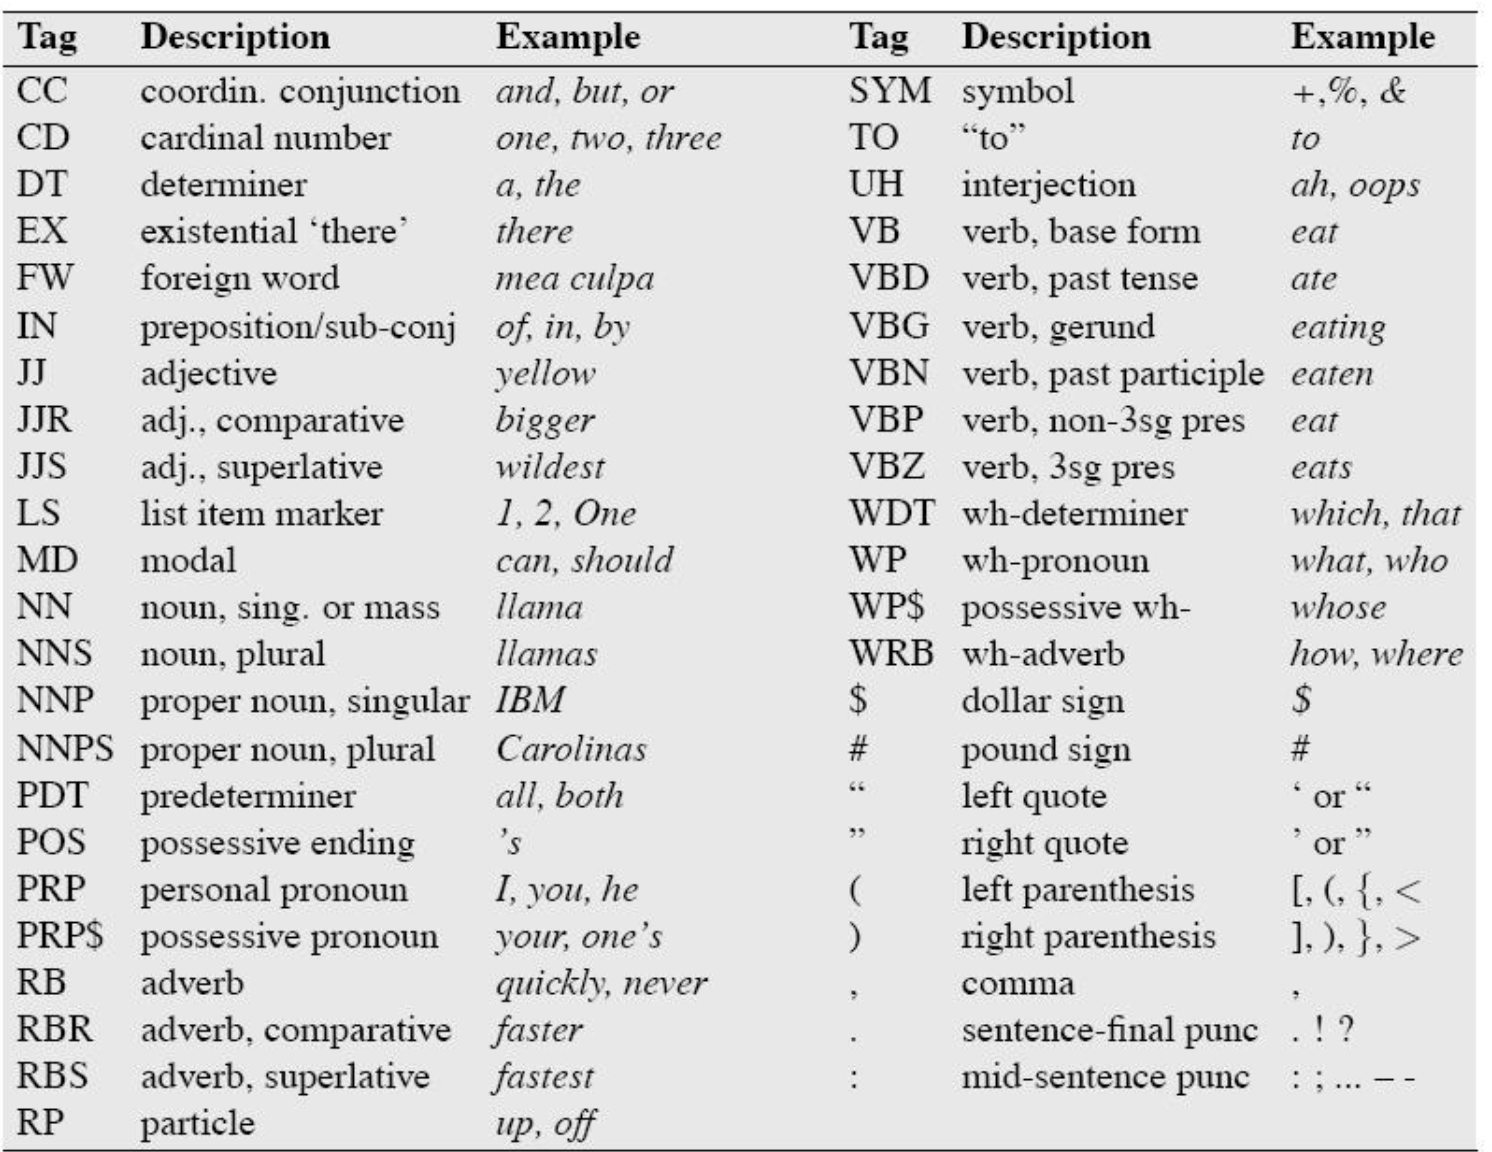
\includegraphics[height=7cm]{w.png}
\\
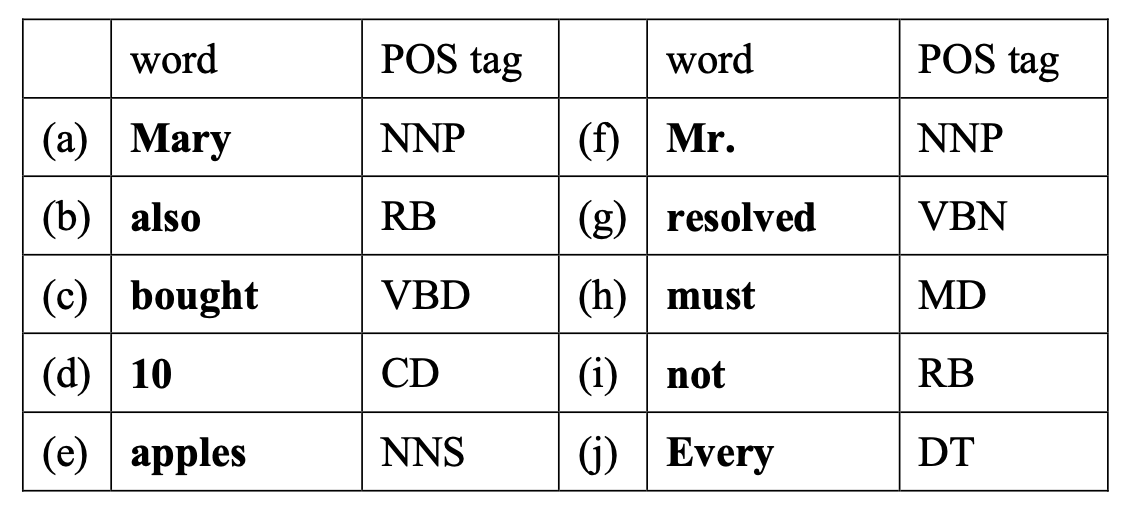
\includegraphics[height=3cm]{w1.png}
\subsection{Personal pronoun}
PRP - He
\subsection*{Determiners (DT)}
the, a, some\\
E.g. Does that\\\\
particles (RP) can appear after object\\
prepositions (IN) can appear only after verb \\
E.g. of, off, on\\
I thought that/IN
\subsection*{adjectives (JJ)} 
E.g. other, grand, already married/JJ
\subsection*{Verbs}
VBD - commented\\
VBP - do, have\\
VBZ - is\\
There/EX are 70 children there/RB
\subsection*{Modal}\\
MD - could\\
\subsection*{Personal Pronouns}
PRP - you\\
PRP\$ - your
\subsection*{Binary classification}
sign(x) = 1 for x $\geq$ 0, -1 for x $<$ 0
Feature extraction so that there is a good mapping of x
\subsection*{Softmax}
[2 -1 5]\\
\(\frac{e^{2}}{e^{2} + e^{-1} + e^{5}}\) into another vector of 3 numbers where it sum to 1
\\
\subsection*{Loss functions}
$L_{cross-entropy} (\hat{y}, y) = - \sum\limits_{i} y log (\hat{y})$\\
\\
or $- log(\hat{y}) for hard classification$\\
$\hat{y}$ is 1 then it can minimize the loss function\\
$\hat{y}$ requires softmax for transformation\\
\subsection*{Ranking loss}\\
$L_{ranking} (x, x') = max(0, 1 - (f(x) - f(x')))$
\subsection*{Gradient descent}
$w_{i} \leftarrow w_{i} - \alpha \frac{\partial_{L}}{\partial_{w_{i}}}$ for $\alpha >$ 0\\
Successive iterative approximation, can't plug in a value like $w_{1, 1}$\\
if L(w) is convex (single min point), then it will converge to global minimum
\subsection*{Expected number of bits}
\sum bits * P(bits) = $1 \times \frac{1}{2} + 2 \times \frac{1}{4} + 3 \times \frac{1}{8}$ ... = 2
Entropy is the number of bits needed to encode
\subsection*{Per word cross entropy} 
Entropy rate = $\frac{1}{n} H(w_{1}) = -\frac{1}{n} (\sum p(W) log(p(W))$
\subsection*{Smoothing}
$P(w|c_{i}) = \frac{\# times\ w\ occur\ in\ texts\ of\ class\ c_{i}}{\sum \# times w\ occurs\ in\ texts\ of\ class\ c_{i}}$
\\
$P(w|c_{i}) = \frac{\# times\ w\ occur\ in\ texts\ of\ class\ c_{i}\ + 1}{\sum \# times\ w\ occurs\ in\ texts\ of\ class c_{i} + V}$\\
$C^{*}(w_{0} w) = \{C(w_{0} w) + 1\} \times \frac{C(w_0)}{C(w_0) + V} $
\\
\subsubsection*{Witten Bell}
\\
If C^{*}($w_{x}w_{i}$) $>$ 0, $C(w_{x})$ $\times \frac{C(w_{x}w_{i})}{C(w_{x}) + T(w_{x})}$
\\
If C^{*}($w_{x}w_{i}$) $=$ 0, $\frac{ c(w_{x})T(w_{x})}{Z(w_{x}) (c(w_{x}) + T(w_{x}))} $
\subsection*{Stochastic POS tagging}
\)\)
 $P(T,W) = P(<s> , t_{1}, w_{1}, t_{2}, w_{2}...<s>)$\\
= $P(<s>) \cdot P(t_{1} | <s>) \cdot P(w_{1} | <s>, t_{1}) $
\\
$P(T|W) = \frac{P(T, W)}{P(W)} = P(T, W)$
\subsection*{Markov assumption}
$w_{k}$ only depends on the previous n - 1 words\\
$P(w_{k} | w_{1}, .., w_{k-1})$ \approx $P(w_{k}| w_{k-1})$
\subsection*{Vertibi}
v(tag, word) = P(w_{i} | t_{i}) \times P(t_{i} | t_{i-1}) \times P(t_{i-1}) \\
\\
Trigram P(t_{i} |  t_{i-1} t_{i-2}) = P(t_{i} |  t_{i-1} t_{i-2}) + P(t_{i} |  t_{i-1}) + P(t_{i})
\subsection*{Forward computation}
1. Look at the number of input nodes\\
2. Compute the s node which is the value before there is actually $h_{1}$(non-linear activation function)\\\\
$s_{i} = w_{x}i_{i} + w_{x+1}i_{i+1} ... + w_{k}i_{k} + ... b_{i}$\\
For the hidden layers $i_{i}$ will be $h_{i}$\\\\
$h_{i} = \frac{1}{1 + e^{-s_{i}}}$\\
Final value $h_{i}$ will be $o_{i}$
\\\\
$L = \frac{1}{2} \big[ (o_{1} - t_{1})^2 +  (o_{2} - t_{2})^2 \big]$\\
\subsection*{Backward computation}
\textbf{Base case}\\
1. Take the s values previously computed \\
2. Calculate $\frac{\partial_{L}}{\partial_{w_{m}}} =  \frac{\partial_{L}}{\partial_{s_{1}}}\frac{\partial_{s_{1}}}{\partial_{w_{m}}}$\\
	E.g. $\frac{\partial_{L}}{\partial_{w_{6}}}$\\
	\\$\frac{\partial_{L}}{\partial_{s_{3}}}= (o_{1} - t_{1}) \times o_{1}(1 - o_{1})$\\
$\frac{\partial_{s_{3}}}{\partial_{w_{6}}} = h_{1}$\\\\
\textbf{Recursive case}\\
E.g. $\frac{\partial_{L}}{\partial_{w_{2}}}$\\
\\$\frac{\partial_{L}}{\partial_{w_{2}}}= \frac{\partial_{L}}{\partial_{s_{1}}} \times i_{2}$\\
$\frac{\partial_{L}}{\partial_{s_{1}}} = \big[\frac{\partial_{L}}{\partial_{s_{3}}} \times w_{5} + \frac{\partial_{L}}{\partial_{s_{4}}} \times w_{7} \big] \times h_{1}(1 - h_{1})$\\
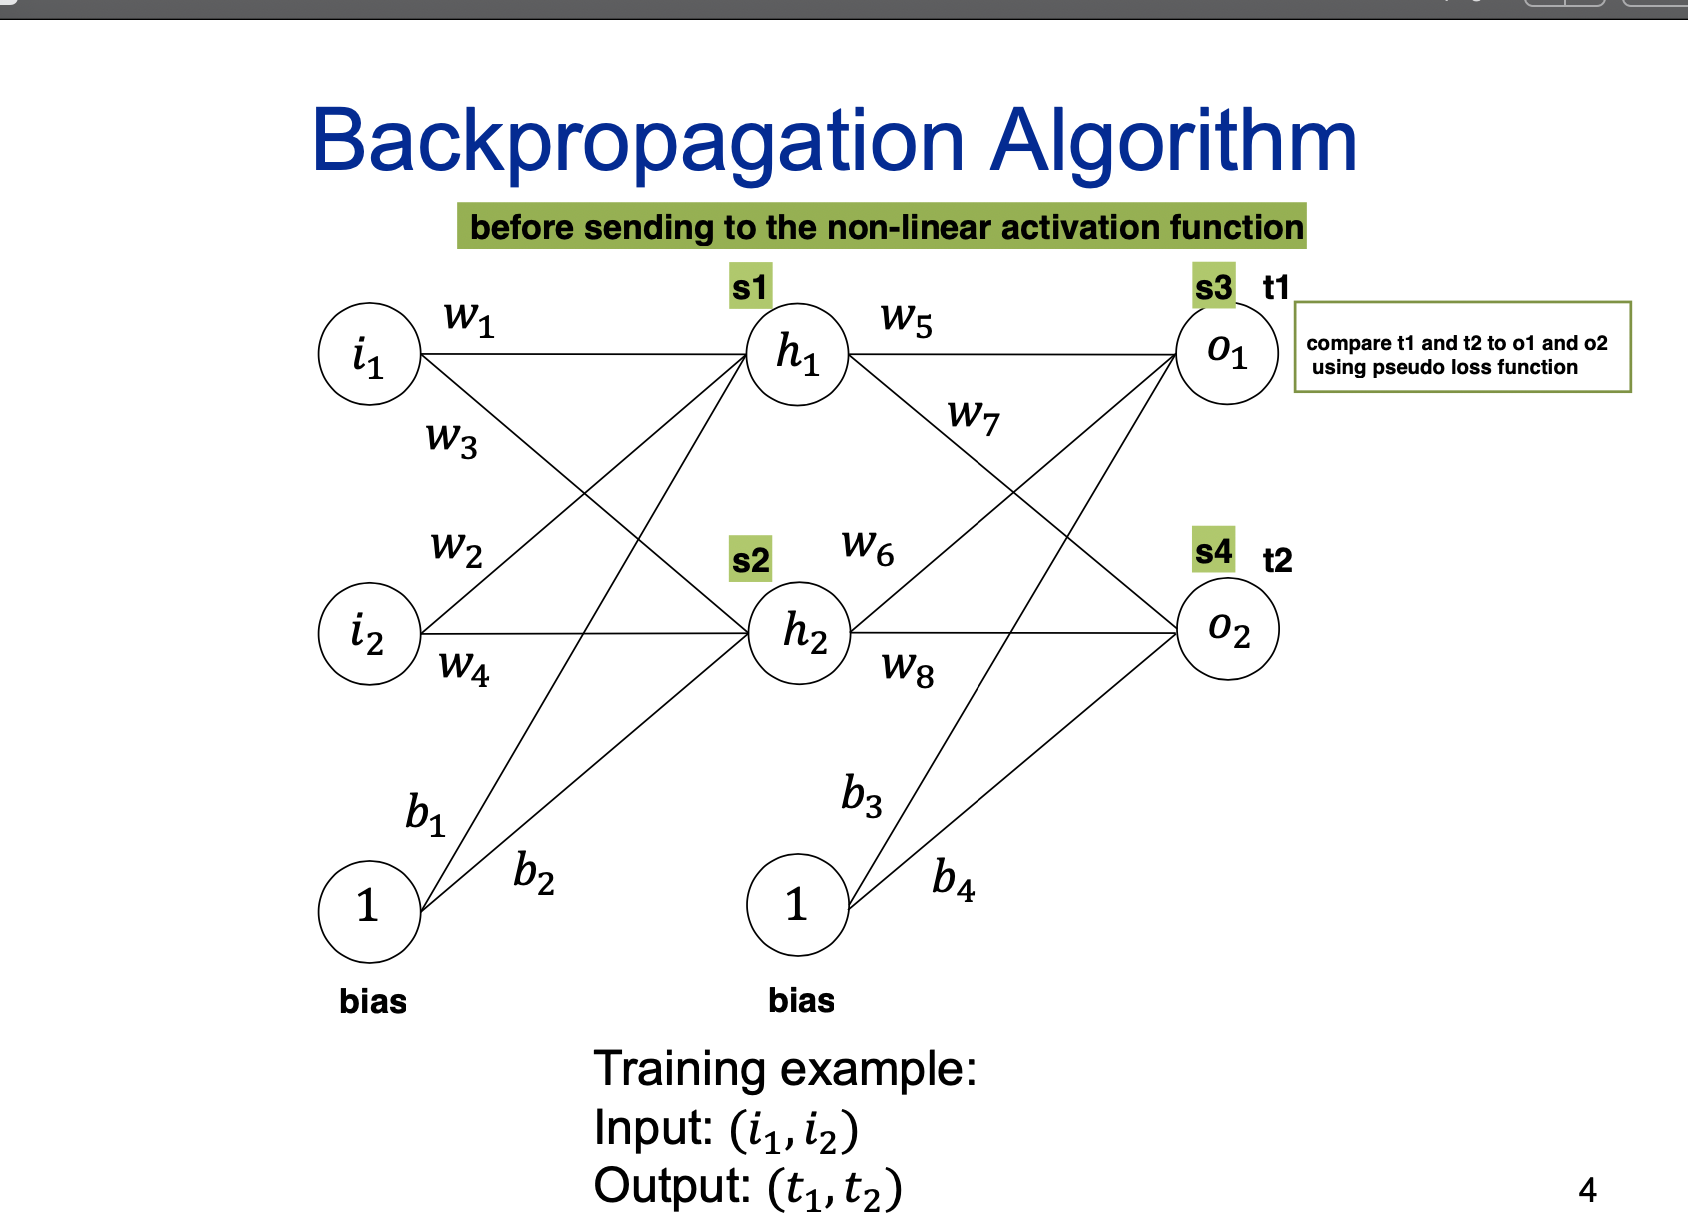
\includegraphics[height=7cm]{b}
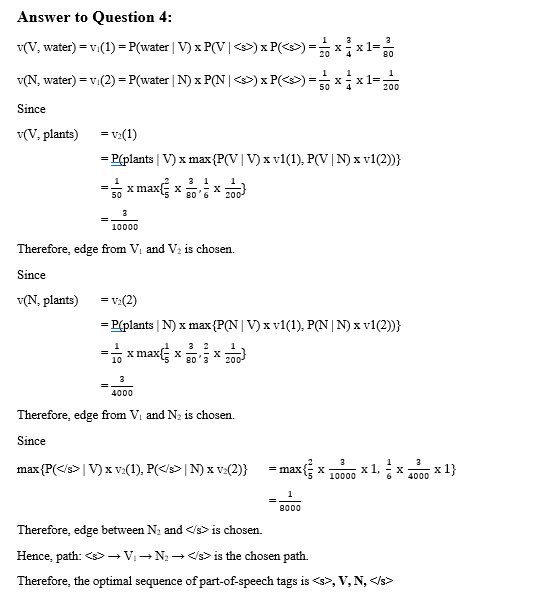
\includegraphics[height=10cm]{ver}
\end{multicols*}

\end{document}
